\documentclass{article}
\usepackage[T1]{fontenc}
\usepackage{lmodern}
\usepackage{graphicx}
\usepackage{amsmath,amssymb}
\usepackage[a4paper,margin=2cm]{geometry}
\usepackage[absolute,overlay]{textpos}
\setlength{\TPHorizModule}{1mm}
\setlength{\TPVertModule}{1mm}
\usepackage[indonesian]{babel}
\usepackage{hyperref}
\setlength{\emergencystretch}{2em}
% unit: Halaman 60

\begin{document}

% === Halaman 60 (python/native) ===

Cipher Berulang (Iterated Cipher)

• Untuk menghasilkan cipher yang lebih kuat, maka dilakukan enciphering sejumlah 

kali (sejumlah putaran) .

• Caranya adalah dengan melakukan berulang kali suatu fungsi transformasi f 

(disebut juga fungsi  putaran atau round function) yang mengubah blok plainteks 

menjadi blokcipherteks. 

• Pada setiap putaran digunakan upa-kunci (subkey) atau kunci putaran (round key) 

yang dikombinasikan dengan plainteks.

60

% deskripsi: gambar native xref 239
\noindent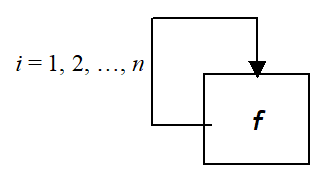
\includegraphics[width=0.85\textwidth]{../../images/python/page_060_img_01.png}

\end{document}
